\documentclass[coverpage]{inftechrep}

\usepackage{comment}

\usepackage{graphicx}
\usepackage{subfigure}
\usepackage{url}

\usepackage{paralist}
\usepackage{hyperref}
\usepackage[all]{hypcap}
\usepackage{verbatim}
\usepackage{array}
\usepackage{float}
\usepackage{multirow}
% \usepackage{rotating}
\usepackage{multicol}
\usepackage{longtable}
\usepackage{changepage}

\usepackage{color}
\usepackage{listings}   
% "define" Scala
\lstdefinelanguage{scala}{
  morekeywords={abstract,case,catch,class,def,%
    do,else,extends,false,final,finally,%
    for,if,implicit,import,match,mixin,%
    new,null,object,override,package,%
    private,protected,requires,return,sealed,%
    super,this,throw,trait,true,try,%
    type,val,var,while,with,yield},
  otherkeywords={=>,<-,<\%,<:,>:,\#,@},
  sensitive=true,
  morecomment=[l]{//},
  morecomment=[n]{/*}{*/},
  morestring=[b]",
  morestring=[b]',
  morestring=[b]"""
}

% A comment in a draft (shouldn't appear in the final version).
\newcommand{\mycomment}[1]{\(\spadesuit\){\bf #1 }\(\spadesuit\)}
% Comment this out in the draft
% \newcommand{\mycomment}[1]{}
\newcommand{\pmcomment}[1]{\comment{PM}{#1}}
\newcommand{\pwtcomment}[1]{\comment{PT}{#1}}
\newcommand{\rscomment}[1]{\comment{RS}{#1}}

% line break in table.  e.g.
% Foo bar & \specialcell{Foo\\bar} & Foo bar \\    % vertically centered
% Foo bar & \specialcell[t]{Foo\\bar} & Foo bar \\ % aligned with top rule
\newcommand{\specialcell}[2][c]{%
  \begin{tabular}[#1]{@{}c@{}}#2\end{tabular}}

  

\begin{document}
\title{Statically Typed Reliability \\Type-parametrized Actors and Their
Supervision (v.0)
}
\author{Jiansen HE}
% \reportnumber{25}
% \reportyear{1999}
% \reportmonth{5}
\keywords{actor, type, supervision tree, nameserver}
% \published{Presented at the WITCH99 Conference, Debrecen, Hungary, May 1999.}
\institutes{
  Laboratory for Foundations of Computer Science}
\maketitle

\begin{abstract}
Building robust concurrent programs, especially in distributed settings, is
challenging as it often involves complex program structures and dynamic
behaviours.  The robustness of concurrent programs could be improved by
\begin{inparaenum}[(i)]
 \item using static type checking to prevent certain data misuses, or
 \item employing failure recovery mechanisms such as supervision tree.
\end{inparaenum}
An important open question is to what extent those approaches could be merged.

This paper presents the design, implementation and preliminary evaluation
results of the TAkka library, where types of actor related components are
statically typed and operations are type checked at the earliest possibility.
We introduce actors parametrized by the type of messages they expect to
receive. We show that it is straightforward to construct
supervision trees of type-parametrized actors. We minimize the number of system
messages that may be handled by general users by providing standard supervision
strategies.

We evaluate the TAkka library by re-implementing 19 examples from other
OTP-like libraries.  our results show that TAkka has small runtime and
code size overheads compared with Akka. Finally, TAkka programs have similar
scalability comparing
to their Akka equivalent.

\mycomment{rewrite the abstract to reflect the purpose of this technical report.}

\mycomment{Let's show how static and dynamic type checking improve actor
programming}

\end{abstract}

\section{Project Description}

\subsection{Background and Motivation}

Concurrent programming is facing new challenges due to the recent advent of multi-core processors, which rely on parallelism, and the pervasive demands of web applications, which rely on distribution.  Theoretic works on concurrency can be traced back to Petri net and other approaches invented in 1960s \cite{historyPA}.  Since 1980, more attention has been paid to the study of process calculi (a.k.a. process algebras), which provide a family of formal models for describing and reasoning about concurrent systems \cite{abramsky}.  The proliferation of Process Calculi marks the advance in concurrency theory.  ``The Dreams of Final Theories'' \cite{abramsky} for concurrency, however, have not been achieved.

In practice, it is difficult to build a reliable distributed system because of its complexity.  Firstly, a distributed system shares features and problems with other concurrent systems.  For instance, it is non-deterministic so that traditional input-output semantics is inadequate to be used for reasoning about its behaviour.  Secondly, scalability of a distributed system is usually a challenge for its developers.  For example, developers of a distributed system are unlikely to know the structure of the system in advance.  Moreover, the mobility \cite{MobileAmbients} of a distributed system requires the capability of changing its topological structure on the fly.  In addition, the latency of communication could be affected by many unpredictable factors.  Thirdly, the system should be tolerant of partial failures.  For example, when a site fails to respond to messages,  the system should address this failure by invoking a recovery mechanism.   	

Fortunately, some recent works provide a solid basis for the design of distributed programming languages.  For example, the ambient calculus \cite{MobileAmbients} models the movement of processes and devices.  Bigraphs \cite{bigraph_book}, a more abstract model, is aiming at describing spatial aspects and mobility of ubiquitous computing.  Session types \cite{Honda93typesfor, Honda_languageprimitives} guarantees that two parties of a session always communicate in a dual pattern.  Lastly, the join-calculus \cite{full_join} is a remarkable calculus which models features of distributed programming as well as provides a convenient construct, the join patterns, for resources synchronisation.  It is also important to note that the syntax of the join-calculus is close to a real programming language and therefore reduces the barrier between understanding the mathematical model and employing this abstract model to guide programming practices.

In addition, good programming principles, such as the OTP design principles\footnote{OTP is stand for Open Telecom Platform.  It provides a set of libraries for developing Erlang applications.  For the above reason, it is also known as Erlang/OTP design principles}, have been developed and verified by the long-term implementation practice.  OTP is a platform for developing concurrent, distributed, fault tolerant, and non-stop Erlang applications \cite{Erlang}.  In the past 20 years, the Erlang language was used to build large reliable applications like RabbitMQ, Twitterfall, and many telecommunications systems.

Nevertheless, Erlang is an untyped functional programming language whereas a typed language detects certain forms of data misuse earlier.  Therefore, it would be pleasant to combine advantages of static typing and OTP principles.  At the time of this writing, this idea has been partly realised in the akka framework \cite{akka}.  In spite of some attempts, the akka framework inherits some limitations of using untyped actors from the Erlang programming language.  This situation left us research potentials in this line.

\subsection{Project Aim}
\label{aim}
The aim of this project is to {\it{build a library that supports OTP design principles in a typed setting}}. The project intends to explore factors that encourage programmers to employ good programming principles.  This project will demonstrate how types and appropriate models help the construction of reliable distributed systems.

\subsection{Project Objectives}
\label{objectives}

\begin{enumerate}
  \item To identify a number of medium-sized applications implemented in Erlang using OTP principles.  Those examples will be served as references to evaluate frameworks that support OTP principles.  Candidate examples shall cover a wide range of aspects in distributed programming, including but not limited to 
    \begin{inparaenum} [(a)]
      \item transmitting messages and potentially computation closures, 
      \item modular composition of distributed components, 
      \item default and extensible failure recovery mechanism, 
      \item eventually consistency model for shared states, and 
      \item dynamic topology configuration and hot code swapping.
    \end{inparaenum} 
  \item To re-implement and compare identified applications within existing frameworks.  The primitives purpose of this work is to be aware of prominent features and limitations of existing frameworks.  As a research which contains certain level of overlaps with other existing and evolving frameworks, this research should distinguish itself from others by devised solutions to some problems which are difficulty to be solved by alternatives.  Moreover, the evaluation component formalised in this work is likely to be novel for comparing frameworks aiming at supporting distributed computation.  The same evaluation component will be used for evaluating our later developed library as well.
  \item To implement a library that supports OTP design principles in a typed setting.  The library could be built either on top of existing frameworks or with lower level constructs.  It important to note that the library might be based on an abstraction that is more general than the actor model.  Although OTP design principles were proposed for the Erlang language, which is based on the Actor model, we believe that it should be possible to rephrase those good programming principles in other models.  To demonstrate the wide applications of OTP design principles, the library interface should provide a certain level of generality so that it could be implemented by and used within different models.
  \item To demonstrate how the proposed library meets the demands of distributed programming.  At this stage, the proposed library will be used to (a) demonstrate how to write small programs aiming at different requirements; (b) demonstrate its scalability of programming in the large by reimplementing applications used in objective 1 and 2.
  \item To summarise some challenges in distributed programming and how to get around those difficulties with the proposed library and other programming frameworks.  The summary will reveal how language libraries, which is used for practical purposes, are related to their theoretical guidance underneath.  It may also plot research blanks for future study.
\end{enumerate}



\section{Actor Programming}
\label{background}

\subsection{Actor Model and OTP Design Principles}

The Actor model defined by Hewitt et al.  \cite{Hewitt:1973} treats actors as
primitive computational components.  Actors collaborate by sending asynchronous
messages to each other.  An actor independently determines its reaction to
messages it receives.

The Actor model is adopted by the Erlang programming language, whose 
developers later summarized 5 OTP design principles to improve the 
reliability of Erlang applications \cite{OTP}.  We notice that the Behaviour 
principle, the Application principle, and the Release principle coincide with 
3 Java and Scala Programming practices listed in Table \ref{otp}.  The 
Release Handling principle requires runtime support for hot swapping.  In a 
platform where hot swapping is not supported in general, e.g. Java Virtual 
Machine (JVM), hot swapping a particular component can be simulated by updating 
the reference to that component. For example, Section \ref{hot_swapping} 
explains how to hot swap the behaviour of an actor in TAkka, which runs on the 
JVM. The Supervision principle, which is the central topic of this paper, 
has no direct correspondence in native JVM based systems.

\begin{table}[t]
\label{otp}
% \tbl{Implementing OTP Design Principles in an OO Language}{
 \begin{center}
\begin{tabular}{| l | p{4.5 cm} | }
\hline
  OTP Design Principle & JAVA/Scala Programming \\
\hline
  Behaviour & defining an abstract class \\
\hline
  Application  & defining an abstract class that has two abstract methods: start and stop \\
\hline
  Release  & packaging related application classes  \\ 
\hline
  Release Handling  & hot swapping support on key modules is required \\
\hline
  Supervision  & no direct correspondence  \\
\hline
\end{tabular}
 \caption[]{Using OTP Design Principles in JAVA/Scala\\  Programming}
\end{center}
%}
\end{table}




\subsection{Akka Actor}
\label{akka actor}


An Akka Actor has four essential components as shown in Figure 
\ref{fig:akka_actor_api}: (i) a receive function that defines its reaction to 
incoming messages, (ii) an actor reference pointing to  itself, (iii) the actor 
 context representing the outside world of the actor, and (iv) the supervisor 
strategy for its children.

\begin{figure}[h]
\label{fig:akka_actor_api}
\begin{lstlisting}[language=scala]
package akka.actor
trait Actor{
  def receive:Any=>Unit
  val self:ActorRef
  val context:ActorContext
  var supervisorStrategy: SupervisorStrategy
}
\end{lstlisting}
\caption{Akka Actor API}
\end{figure}

Figure \ref{akkastring} shows an example actor in Akka.  The {\tt receive} 
function of the Akka actor has type {\tt Any$\Rightarrow$Unit} but the 
defined actor, {\tt ServerActor}, is only intended to process strings.  At Line 
16, a {\tt Props}, an abstraction of actor creation, is initialized and passed 
to an actor system, which creates an actor with name \textcolor{mauve}{\tt 
server} and returns a reference pointing to that actor.  Another way to obtain 
an actor is using the {\tt actorFor} method as shown in line 24.  We then use 
actor references to send the actor string messages and integer messages.  
String messages are processed in the way defined by the receive function.

\begin{figure}[t]
 \label{akkastring}
      \begin{lstlisting}[language=scala]
class ServerActor extends Actor {
  def receive = {
    case m:String => println("received message: "+m)
  }
}

class MessageHandler(system: ActorSystem) extends Actor {
  def receive = {
    case akka.actor.UnhandledMessage(message, sender, recipient) =>
      println("unhandled message:"+message);
  }
}

object ServerTest extends App {
  val system = ActorSystem("ServerTest")
  val server = system.actorOf(Props[ServerActor], "server")
  
  val handler = system.actorOf(Props(new MessageHandler(system)))
  system.eventStream.subscribe(handler,
                     classOf[akka.actor.UnhandledMessage]);
  server ! "Hello World"
  server ! 3
  
  val serverRef = system.actorFor("akka://ServerTest/user/server")
  serverRef ! "Hello World"
  serverRef ! 3
}


/*
Terminal output:
received message: Hello World
unhandled message:3
received message: Hello World
unhandled message:3
*/
    \end{lstlisting}
    \caption{A String Processor in Akka}
\end{figure}

Undefined messages are treated differently in different actor libraries.  In
Erlang, an actor keeps undefined messages in its mailbox, attempts to process
the message again when a new message handler is in use.  In versions prior to
2.0, an Akka actor raises an exception when it processes an undefined message.
In recent Akka versions, an undefined message is discarded by the actor and an
{\tt UnhandledMessage} event is pushed to the event stream of the actor system.
The event stream may be subscribed by other actors who are interested in
particular event messages.  To handle the unexpected integer message in the
above short example, an event handler is defined and created with 6 lines of 
code.


\subsection{Supervision}
\label{akkasup}



Reliable Erlang applications typically adopt the Supervision Principle
 \cite{OTP}, which suggests that actors should be organized in a tree structure 
so that any failed actor can be properly restarted by its supervisor.  
Nevertheless, adopting the Supervision principle is optional in Erlang.

The Akka library makes supervision obligatory by restricting the way of 
creating actors. Actors can only be initialized by using the {\tt actorOf}
method provided by {\tt ActorSystem} or {\tt ActorContext}.  Each actor system
provides a guardian actor for all user-created actors.  Calling the {\tt
actorOf} method of an actor system creates an actor supervised by the 
guardian actor.  Calling the {\tt actorOf} method of an actor context 
creates a child actor supervised by that actor.  Therefore, all user-created  
actors in an actor system, together with the guardian actor of that actor 
system, form a tree structure.  Obligatory supervision unifies the 
structure of actor deployment and simplifies the work of system maintenance.

Each actor in Akka is associated with an actor path.  The string representation
of the actor path of a guardian actor has format 
{\it akka://mysystem@IP:port/user}, where {\it mysystem} is the name of the 
actor system, {\it IP} and {\it port} are the IP address and the 
port number which the actor system listens to, and {\it user} is the name of 
the guardian actor.  The actor path of a child actor is actor path of its 
supervisor appended by the name of the child actor, either a user specified 
name or a system generated name.

Figure \ref{supervisedcalculator} defines a simple calculator which supports
multiplication and division. The simple calculator does not consider the
problematic case of dividing a number by 0, where an {\tt
ArithmeticException} will be raised.  We then define a safe calculator as the 
supervisor of the simple calculator.  The safe calculator delegates 
calculation tasks to the simple calculator and restarts the simple calculator 
when an {\tt ArithmeticException} is raised.  The supervisor strategy of
the safe calculator also specifies the maximum number of failures its child may 
have within a given time range.  If the child fails more frequently than the 
allowed frequency, the safe calculator will be  stopped, and its failure will be
reported to its supervisor, the system guardian actor in this example.  The
terminal output shows that the simple calculator is restarted before the third 
message and the fifth message are delivered.  The last message is not processed
because both calculators are terminated since the simple calculator fails more 
frequently than allowed.

\begin{figure}
\label{supervisedcalculator}

  \begin{lstlisting}[language=scala]
case class Multiplication(m:Int, n:Int)
case class Division(m:Int, n:Int)

class Calculator extends Actor {
  def receive = {
    case Multiplication(m:Int, n:Int) =>
      println(m +" * "+ n +" = "+ (m*n))
    case Division(m:Int, n:Int) =>
      println(m +" / "+ n +" = "+ (m/n))
  }
}

class SafeCalculator extends Actor {
  override val supervisorStrategy =
    OneForOneStrategy(maxNrOfRetries = 2, withinTimeRange = 1 minute) {
      case _: ArithmeticException  =>
        println("ArithmeticException Raised to: "+self)
        Restart
    }
  val child:ActorRef = context.actorOf(Props[Calculator], "child")
  def receive = {
    case m => child ! m
  }
}

  val system = ActorSystem("MySystem")
  val actorRef:ActorRef = system.actorOf(Props[SafeCalculator],
"safecalculator")

  calculator ! Multiplication(3, 1)
  calculator ! Division(10, 0)
  calculator ! Division(10, 5)
  calculator ! Division(10, 0)
  calculator ! Multiplication(3, 2)
  calculator ! Division(10, 0)
  calculator ! Multiplication(3, 3)

/*
Terminal Output:
3 * 1 = 3
java.lang.ArithmeticException: / by zero
ArithmeticException Raised to: Actor[akka://MySystem/user/safecalculator]

10 / 5 = 2
java.lang.ArithmeticException: / by zero
ArithmeticException Raised to: Actor[akka://MySystem/user/safecalculator]
java.lang.ArithmeticException: / by zero

3 * 2 = 6
ArithmeticException Raised to: Actor[akka://MySystem/user/safecalculator]
java.lang.ArithmeticException: / by zero
*/
    \end{lstlisting}
  \caption{Supervised Calculator}
\end{figure}
\section{Adding Type Parameter to Actor Library}

This section examines actor programming in the Akka library and how type parameters are added to actor-related classes to improve type safety.  We show that supervision trees in TAkka are constructed in the same way as in Akka.  This section concludes with a brief discussion about alternative designs used by Akka and other actor libraries.

\mycomment{Explain Actor Programming.  Compare Akka and TAkka side by side.}

\subsection{The Actor Class}

An Actor has four important fields given in Figure-\ref{actor_api}:
(i) a receive function that defines its reaction to incoming messages, (ii)
an actor reference pointing to  itself, (iii) the actor  context representing
the outside world of the actor, and (iv) the supervisor strategy for its
children.


An TAkka {\bf Actor} has Akka equivalent fields as shown in
Table \ref{actor_api}.  Different from other actor libraries, every TAkka
actor class takes a type parameter {\bf M} which specifies the type of messages
it expects to receive.  The same type parameter is used as the input type of the
receive function, the type parameter of actor context and the type parameter of
the actor reference pointing to itself.  We introduce a new field $mt$ to inform the compiler that the type parameter of the {\bf Actor} class should be recorded.

\begin{table}[h]
\label{actor_api}
\caption{Akka and TAkka Actor}
%  \begin{adjustwidth}{-1.8cm}{}
  \begin{tabular}{ l   l }
\begin{lstlisting}[language=scala]
package akka.actor
trait Actor {

  def typedReceive:Any=>Unit
  val typedSelf:ActorRef
  val typedContext:ActorContext
  var supervisorStrategy:
         SupervisorStrategy
}
\end{lstlisting} &
\begin{lstlisting}[language=scala]
package takka.actor
trait Actor[M] {
  implicit val mt : TypeTag[M]
  def typedReceive:M=>Unit
  val typedSelf:ActorRef[M]
  val typedContext:ActorContext[M]
  var supervisorStrategy: 
         SupervisorStrategy
}
\end{lstlisting}
  \end{tabular}
%  \end{adjustwidth}
\end{table}



The three immutable fields of TAkka {\bf Actor}: {\it mt}, {\it typedContext} and {\it
typedSelf}, will be initialised automatically when the actor is created.
Application developers may override the default supervisor strategy in the way
explained in \S\ref{supervision}.  The implementation of the {\it typedReceive}
method, on the other hand, is left to developers.


\subsection{Actor Reference}
\label{actor_ref}
A reference pointing to an Actor of type {\bf Actor[M]} has type {\bf ActorRef[M]}.  It provides a {\it !} method, through which users could send a message of type {\bf M} to the referenced actor.  Sending an actor reference a message whose type is not the
expected type will raise a compile error.  By using type-parametrized actor
references, the receiver does not need to worry about unexpected messages while
senders can ensure that messages will be understood and processed, as long as
the message is delivered.

In a type system which supports polymorphism, {\bf ActorRef} should be
contravariant.  We further provide a {\it publishAs} method which type-safely
casts an actor reference to a version of its supertype.  In another word, the
output actor reference accepts partial forms of messages that are accepted by
the input actor reference.  The ability of publishing partial services makes
TAkka a good tool for solving security problems such as the type pollution
problem described at \S\ref{type_pollution}.

\begin{table}[h]
\label{ActorRef}
  \begin{tabular}{ l  l }
      \begin{lstlisting}[language=scala]
abstract class ActorRef {

  def !(message: Any):Unit
  
  
}
    \end{lstlisting} 
    &
    \begin{lstlisting}[language=scala]
abstract class ActorRef[-M]
    (implicit mt:TypeTag[M]) {
  def !(message: M):Unit
  def publishAs[SubM<:M]
      (implicit mt:TypeTag[SubM]):ActorRef[SubM]
}
    \end{lstlisting}     
  \end{tabular}
    \caption{Actor Reference}
\end{table}

The code below defines and uses a string processing actor in Akka and TAkka.  The receive
function of Akka Actor has type {\bf Any$\Rightarrow$Unit} but the defined actor
only intends to process strings. Both examples create an actor inside an actor system
and returns a reference pointing to that actor.  The same string message is sent to actor in both examples
and processed in the way defined in the receive function.  Sending an integer message, which is not expected
by both actors; However, is permitted in the Akka version but rejected by the TAkka version.

\begin{table}[h]
\label{ActorRef}
     \begin{adjustwidth}{-0.8cm}{}
  \begin{tabular}{ l   l }
      \begin{lstlisting}[language=scala]
class MyActor extends Actor {
  def receive:Any => Unit = {
    case m:String =>
      println("Received message: " + m)
  }
}

val system = ActorSystem("MySystem")
val actorRef:ActorRef =
    system.actorOf(Props[MyActor])
actorRef ! "Hello World!"
actorRef ! 3



/*
Terminal output:
Received message: Hello World!
*/
    \end{lstlisting}
&
      \begin{lstlisting}[language=scala]
class MyActor extends Actor[String] {
  def typedReceive:String=>Unit = {
    case m:String =>
      println("received message: "+m)
  }
}

val system = ActorSystem("MySystem")
val actorRef:ActorRef[String] = 
    system.actorOf(Props[String, MyActor])
actorRef ! "Hello World!"
// actorRef ! 3 
// compile error: type mismatch; found : Int(3)
//   required: String

/*
Terminal output:
Received message: Hello World!
*/
    \end{lstlisting}

  \end{tabular}
  \end{adjustwidth}
    \caption{A Actor String Processor}
\end{table}

Undefined messages are treated differently in different actor libraries.  In
Erlang, an actor keeps undefined messages in its mailbox, attempts to process
the message again when a new message handler is in use.  In versions prior to
2.0, an Akka actor raises an exception when it processes an undefined message.
In recent Akka versions, undefined message is discarded by the actor and an {\bf
UnhandledMessage} event is pushed to the event stream of the actor system. The
event stream may be subscribed by other actors to which all events will be
published.  In the example code no subscriber of the event stream is defined and
the integer message is simply discarded.


\subsection{Props and Actor Context}
\label{actor_context}
\mycomment{Explain Akka version and TAkka version at the same time}

A Props is the configuration of actor creation.  A Props of type {\bf Prop[M]}
specifies how to create an actor of type {\bf Actor[M]} and returns an actor
reference of type {\bf ActorRef[M]}.  A Prop should be created by one of
following APIs, where {\bf MyActor} should be a subtype of {\bf Actor[M]}:

\begin{table}[h]
\label{Props}
     \begin{adjustwidth}{-1.2cm}{}
  \begin{tabular}{ l  l }

\begin{lstlisting}[language=scala]
 val props:Props = Props[MyActor]
 val props:Props = Props(new MyActor)
 val props:Props = Props(myActor.getClass)
\end{lstlisting}
&
\begin{lstlisting}[language=scala]
 val props:Props[M] = Props[M, MyActor]
 val props:Props[M] = Props[M](new MyActor)
 val props:Props[M] = Props[M](myActor.getClass)
\end{lstlisting}
  \end{tabular}
     \end{adjustwidth}
    \caption{Props Creation API}
\end{table}
  

Contrary to actor reference, an actor context describes the outside world of the
actor.   For security consideration, actor context is only available inside the
actor definition.  By using APIs in Figure \ref{ActorContext}, an actor can (i)
retrieving an actor reference according to a given actor path, (ii) creating a
child actor with system generated or user specified name, (iii) set a timeout
during which period a new message shall be received, and (iv) update its
behaviours.

The {\it ActorFor} method in the {\bf ActorContext} classes returns an actor
reference of the desired type, if the actor located at the specified actor path
has a compatible type.  To implement the {\it ActorFor} method, we would like to
have a more general mechanism that will return a value of the desired type
when the corresponding key is given.  To this end, we designed and implemented a
typed name server which will be explained \S\ref{nameserver}.

The {\it become} method enables hot code swap on the behaviour of an actor.  The
{\it become} method in TAkka is different from code swap in Akka in two aspects.
 Firstly, the supervision strategy could be updated as well.  Secondly, the new
receive function must be more general than the previous version.  As a result,
no stack of receive functions is required.  Interestingly, the implementation of
{\it become} involves a mix of static and dynamic type checks.  Details of the
implementation will be discussed in \S\ref{code_evolution}.

\begin{table}[h]
\label{ActorContext}
   \begin{adjustwidth}{-1.3cm}{}
  \begin{tabular}{ l   l }
      \begin{lstlisting}[language=scala]
trait ActorContext {
  def actorFor(actorPath:String):ActorRef
  
  def actorOf(props: Props):ActorRef
  def actorOf(props: Props, 
              name: String): ActorRef
  def setReceiveTimeout
             (timeout: Duration): Unit

  def become(
      newReceive: Any => Unit,
  ):ActorRef
}



    \end{lstlisting}
&
    \begin{lstlisting}[language=scala]
trait ActorContext[M] {
  def actorFor [Msg] (actorPath: String)
       (implicit mt: TypeTag[Msg]): ActorRef[Msg]
  def actorOf[Msg](props: Props[Msg])
        (implicit mt: TypeTag[Msg]): ActorRef[Msg]
  def actorOf[Msg](props: Props[Msg], name: String)
        (implicit mt: TypeTag[Msg]): ActorRef[Msg]
  def setReceiveTimeout(timeout: Duration): Unit

  def become[SupM >: M](
      newTypedReceive: SupM => Unit,
      newSystemMessageHandler:
                         SystemMessage => Unit,
      newSupervisionStrategy:SupervisionStrategy
  )(implicit smt:TypeTag[SupM]):ActorRef[SupM]
}
    \end{lstlisting}
    \end{tabular}
     \end{adjustwidth}
    \caption{Actor Context}
\end{table}


\subsection{Supervision Strategies}
\label{supervision}

There are three supervision strategies defined in Erlang/OTP: one-for-one,
one-for-all, and rest-for-one\cite{OTP}.  If a supervisor adopts the one-for-one
supervision strategy, a child will be restarted when it fails.  If a supervisor
adopts the one-for-all supervision strategy, all children will be restarted when
any of them fails.  In Erlang/OTP, children are started in a user-specified
order.  If a supervisor adopts the rest-for-one supervision strategy, all
children started after the failed child will be restarted.  For each
supervision strategy, users can further specify the maximum restarts of any
child within a period.

The Akka library only considers the one-for-one strategy and the one-for-all
strategy.  The rest-for-one strategy is not considered because children are not
created according to a user-specified order.  The default supervision strategy
is a one-for-one strategy that permits unlimited restarts.  Users can define
their own supervision strategy by using APIs given in Figure-\ref{super}.  {\bf
OneForOne} corresponds to the one-for-one strategy in Erlang whereas {\bf
OneForAll} corresponds to the all-for-one strategy in Erlang.  Both
strategies are constructed by providing required parameters.  {\bf Directive} is
an enumerable type whose value is {\bf Escalate}, {\bf Restart}, {\bf Resume},
or {\bf Stop}.  Notice that neither supervision strategies require any type-parametrized class. Therefore, both supervision strategies
are constructed in TAkka in the same way as in Akka.


\begin{figure}[h]
\label{super}
    \begin{lstlisting}    
abstract class SupervisorStrategy
case class OneForOne(restart:Int, time:Duration)
                    (decider: Throwable => Directive) extends SupervisorStrategy
case class OneForAll(restart:Int, time:Duration)
                    (decider: Throwable => Directive) extends SupervisorStrategy
    \end{lstlisting}
    \caption{Supervision Strategies}
\end{figure}


\subsection{Handling System Messages}

Actors are communicated with each other by sending messages.  To maintain a
supervision tree, for example to monitor and control the liveness of actors, a
special category of messages should be addressed by all actors.  We define a
trait {\bf SystemMessage} to be the supertype of all messages for system
maintenance purposes.  Based on the design of Erlang and Akka, we consider
following messages should be included in system messages:

\begin{itemize}
  \item {\bf ChildTerminated(child: ActorRef[M])}  

  a message sent from a child actor to its supervisor before it terminates.

  \item {\bf Kill}

  a message sent from a supervisor to its child.

  \item {\bf Restart}
 
  a message sent from a supervisor to its terminated child asking to restart the child.

  \item {\bf ReceiveTimeout}

  a message sent from an actor to itself when it did not receive any message after a timeout.

\end{itemize}

An open question is which system messages are allowed to be handled by users.
In Erlang and early Akka versions, all system messages could be explicitly
handled by users in the {\it receive} block.  In recent Akka versions, there is
a consideration that some system messages should be handled in library
implementation but not be handled by library users.

Considering that there are only two supervision strategies to consider, both of
which have clearly defined operational behaviours, all messages related to the
liveness of actors are handled in the TAkka library implementation.  General
library users may indirectly affect the system message handler via specifying
the supervision strategies.  On the contrary, messages related to the behaviour
of an actor, e.g. ReceiveTimeout, are better to be handled by application
developers.  In TAkka, {\bf ReceiveTimeout} is the only system message that can
be explicitly handled by users.

\subsection{Alternative Designs}
\label{alternative designs}


\paragraph{Akka Typed Actor}
In the Akka library, there is a special class called {\bf TypedActor}, which
contains an internal actor and could be supervised.  Users of typed actor invoke
a service by calling a method instead of sending messages.  The typed actor
prevents some type errors but has two limitations.  For one thing, typed actor
does not permit code evolution.  For the other, avoiding type pollution when
using typed actor would be as awkward as using a plain objected-oriented model.

\paragraph{Actors with or without Mutable States}
The actor model formalised by Hewitt et al. \cite{Hewitt:1973} does not specify
its implementation strategy.  In Erlang, a functional programming language,
actor does not have mutable states.  In Scala, an objected-oriented
programming language, actor may have mutable states.  The TAkka library is
built on top of Akka and implemented in Scala as well.  As a result, TAkka does
not prevent users from defining actors with mutable states.  Nevertheless, the
library designers would like to encourage using actors in a functional
style because actors with mutable states is difficult to synchronize in a
cluster environment.

In a cluster, resources are replicated at different locations to provide
efficient fault-tolerant services.  Known as the CAP theorem \cite{CAP}, it is
impossible to achieve consistency, availability, and partition tolerance in a
distributed system simultaneously.  For actors without mutable state, system
providers do not need to worry about consistency.  For actors that contain
mutable states, system providers have to either sacrifice availability or
partition tolerance, or modify the consistency model.  For example, Akka actor
has mutable states and Akka cluster employs an eventual consistency
model \cite{Kuhn12}.

\paragraph{Linked Actors}
Alternative to forming supervision trees, reliability of actor-based programs
could be improved by linking related actors \cite{ErlangWeb}. Linked actors are
aware of the death of each other.  Indeed, supervision tree is a special
structure for linking actors.  For this reason, we consider actor linking is a
redundant design in a system where supervision is obligatory.  After all, if
the computation of an actor relies on the liveness of another actor, those two
actors should be organised in the same logic supervision tree.






\begin{comment}
\section{Mixing Static and Dynamic Type Checking}

Implementing {\bf ActorContext} described as \S\ref{actor_context} requires a
mixture of static and dynamic type checking.  This section looks into how
static and dynamic type checking are combined to guarantee backward compatible
code evolution and support type safe data retrieval.

\subsection{Backward Compatible Code Evolution}
\end{comment}
\section{Backward Compatible Code Evolution}
\label{code_evolution}

Partial service upgrade is a desired feature of distributed systems, whose
components are typically developed separately. Unfortunately, hot code swap is
not supported by the JVM, the platform where the TAkka library runs on.  To
support hot swapping on an actor's receive function, system message handler, and
supervision strategy, those three behaviour methods are maintained as object
reference.

Different from Erlang and Akka Design, code evolution in TAkka must be backward
compatible.  In another word, an actor must evolve to a version that is able to
handle the same amount of or more message patterns.  The above decision is made
so that a service published to users would not be unavailable later.

\begin{figure}[h]
\label{become}
\begin{lstlisting}
trait ActorContext[M] {
 implicit var mt:Manifest[_] = manifest[M]

 def become[SupM >: M](
      newTypedReceive: SupM => Unit,
      newSystemMessageHandler:
               SystemMessage => Unit
      newSupervisionStrategy:SupervisionStrategy
 )(implicit smt:Manifest[SupM]):ActorRef[SupM] = {
     if (!(smt >:> mt))
       throw BehaviorUpdateException(smt, mt)

    this.mt = smt
    this.systemMessageHandler =  newSystemMessageHandler
    this.timeoutHandler = newTimeoutHandler
    this.supervisionStrategy = newSupervisionStrategy

    // other code
 }
}
\end{lstlisting}
\caption{Code Evolution in TAkka}
\end{figure}

The {\it become} method is implemented as in Figure-\ref{become}.  The manifest
for static type {\bf M} should be interpreted as the least general type of
messages addressed by the actor initialized from {\bf Actor[M]}.  The
manifest for {\bf SupM} will only be known when the {\it become} method is
invoked.  When a series of {\it become} invocations are made at run time, the
order of those invocations may be non-deterministic.  Therefore, performing a
dynamic type checking is required to guarantee backward compatibility.
Nevertheless, static type checking prevents some invalid {\it become}
invocations at compile time.




\section{Library Evaluation}

This section presents preliminary evaluation results of the TAkka library.  
We show that the Wadler's type pollution problem can be strateforwardly avoided by in TAkka.   
We further assess the TAkka library by porting examples built in Erlang and Akka.  The
result shows that TAkka is able to detect more forms of type errors without
obvious overheads.


\subsection{Wadler\rq{}s Type Pollution Problem}
\label{type_pollution}

Wadler\rq{}s type pollution problem refers to the situation where the same
communication interface is published to two or more parties for distinct
purposes.  In a system suffers from the type pollution problem, a service
provider may receive a request that is not expected from the requester.
Examples of type polluted systems are those constructed using the layered
architecture or the MVC model without due care.

One solution to the type pollution problem is using separate channels for
distinct parties.  Programming models that supports this solution includes
join-calculus \cite{full_join} and session types\cite{Honda_languageprimitives}.

The other solution to the type pollution problem is using sub-typing.  Take a
layered architecture system for example. Let {\bf UpperMsg} and {\bf LowerMsg}
be the type of messages expected from the upper layer and the lower layer
respectively.  Both {\bf UpperMsg} and {\bf LowerMsg} are subtypes of {\bf
MiddleMsg}, the least general type of messages expected by the middle layer.
In the code below, the middle layer publishes itself as different types to the
upper layer and the lower layer.  Therefore, neither the upper layer nor the
lower layer is aware of the communication interface between the other
layer and the middle layer.

\begin{lstlisting}
sealed trait MiddleMsg
class UpperMsg extends MiddleMsg
class LowerMsg extends MiddleMsg

class UpperLayer {
  private var middle:ActorRef[UpperMsg]
  def setMiddleLayer(mid:ActorRef[UpperMsg]) = {
    this.middle = mid
}}
class LowerLayer {
  private var middle:ActorRef[LowerMsg]
  def setMiddleLayer(mid:ActorRef[LowerMsg]) = {
    this.middle = mid
}}

class MiddleLayer extends Actor[MiddleMsg] {
  val upper:UpperLayer
  val lower:LowerLayer

  upper.setMiddleLayer(typedSelf)
  lower.setMiddleLayer(typedSelf)
  // rest of initialization code
}
\end{lstlisting}

\subsection{Expressiveness and Correctness}

Table-\ref{express} lists examples used for expressiveness and correctness test.
We selected examples from Akka and other OTP projects and re-implement them  in
TAkka to ensure that main requirements for actor programming are not
unintentionally neglected.  The reported results show that when porting an Akka
program to TAkka, new type declarations will be added to about 12\% lines of
code; Meanwhile, because TAkka actors do not need to handle unexpected messages,
the total program size of Akka and TAkka applications are almost the same.

A type error is reported by the compiler when porting the Socko example
\cite{SOCKO} from its Akka implementation to equivalent TAkka implementation.
SOCKO is a library for building event-driven web services.  The SOCKO designer
defines a {\bf SockoEvent} class to be the supertype of all events.  One
subtype of {\bf SockoEvent} is {\bf HttpRequestEvent}, representing events
generated when an HTTP request is received. The designer further implements
subclasses of {\bf Method}, whose {\it unapply} method intends to pattern
matching {\bf SockoEvent} to {\bf HttpRequestEvent}.  Somehow, the SOCKO
designer made a type error in the method declaration so that the {\it unapply}
method pattern matches {\bf SockoEvent} to {\bf SockoEvent}. The type error is
not exposed in test examples because the designer always passes instances of
{\bf HttpRequestEvent} to the {\it unapply} method and send the the returned
values to an actor that accepts messages of {\bf HttpRequestEvent} type.
Fortunately, such ill-typed message is not accepted in TAkka, even if the code
may or may not work.

\begin{table}[h]
\label{express}
% \tbl{Examples for Correctness and Expressiveness Test}{
\caption{Examples for Correctness and Expressiveness Test}
  \begin{adjustwidth}{-1.8cm}{}
\begin{tabular}{| l | c | c | c |  c | c | c |}
\hline

Source & Example & \specialcell{Akka\\ Code Lines} &
\specialcell{Modified\\ TAkka Lines} & \specialcell{\% of \\Modified Code} &
\specialcell{TAkka\\Code Lines}
& \specialcell{\% of \\Code Size} \\
\hline
Quviq\cite{quviq}  & ATM simulator & 1148 & 199 & 17.3 & 1160 & 101 \\
\cline{2-7}
                   & Elevator Controller &
2850 & 172 & 9.3 & 2878 & 101 \\
\hline


                   & Ping Pong & 67 & 13 & 19.4 & 67 & 100 \\
\cline{2-7}
Akka   & Dining Philosophers &
189 & 23 & 12.1 &
189 & 100  \\
\cline{2-7}
Documentation\cite{akka_doc}  & Distributed Calculator  & 250 &
43 & 17.2 & 250 & 100 \\
\cline{2-7}
                                   & Fault Tolerance & 274 & 69 & 25.2 & 274 &
100 \\
\hline

                                   & Barber Shop\cite{BarberShop} & 754 & 104 &
13.7 & 751 & 99 \\
\cline{2-7}
Other Open & EnMAS \cite{EnMAS} & 1916 & 213
& 11.1 & 1909 &
100 \\
\cline{2-7}
Source Akka        & Socko Web Server \cite{SOCKO} & 5024 & 227
& 4.5 & 5017 & 100 \\
\cline{2-7}
Applications                                          & Gatling \cite{Gatling} 
& 1635 & 111 & 6.8 & 1623 & 99\\
\hline
geometric mean                   & & 712.4 & 83.7 & 12.2 & 712.7 & 100.0 \\
\hline
\end{tabular}
% }
  \end{adjustwidth}
\end{table}




\subsection{Efficiency and Scalability Evaluation}
The TAkka library is build on top of Akka so that code for shared features could
be re-used.  The three main overheads of the TAkka implementation are: (i) the
cost of adding an additional operation layer on top of Akka code, (ii) the cost
of constructing {\bf Manifest}, and (iii) the cost of transmitting {\bf
Manifest} in distributed settings.  The cost of the last factor is subject to
network connections.  We access the upper bound of the cost of the first two
factors by accessing the time of initializing {\it n} instances of {\bf MyActor}
defined in \S\ref{akka actor} and \S\ref{actor_ref}.  When {\it n} ranges from
$10^4$ to $10^5$, the time measurement TAkka implementation is about 30\% more
than the time measurement of Akka implementation.

We further investigated the efficiency and scalability of TAkka by porting
9 examples from the BenchErl benchmarks in the RELEASE project \cite{RELEASE}.
The benchmarks are run on a Beowulf cluster at the Heriot-Watt University.
The 32 Beowulf cluster nodes each comprise eight Intel 5506 cores running at
2.13GHz. All machines running under Linux CentOS 5.5. The Beowulf nodes are
connected with Baystack 5510-48T switch with 48 10/100/1000 ports.  

Figure \ref{scalability} gives the result of three representative benchmarks: MBrot,
RUN, and SerialMsg. Each benchmark spawns one master process and many child
processes.  The child process performs a certain amount of calculation and
reports the result to the master process.  The MBrot example requires heavy
calculation in each child process.  The RUN example requires a small amount of
calculation in each child process.  The SerialMsg example ask each child forward
messages. The result shows that TAkka and Akka have almost identical run-time performance and scalability.  For all 3 examples in Figure \ref{scalability}, TAkka is never more than 10.5\% slower than Akka.

\begin{figure}[h]
     \begin{center}
        \subfigure[]{
            \label{fig:first}
            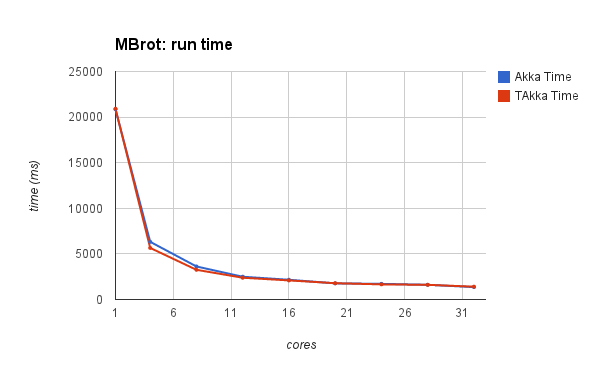
\includegraphics[scale=0.33]{MBrot_time.png}
        }
        \subfigure[]{
           \label{fig:second}
           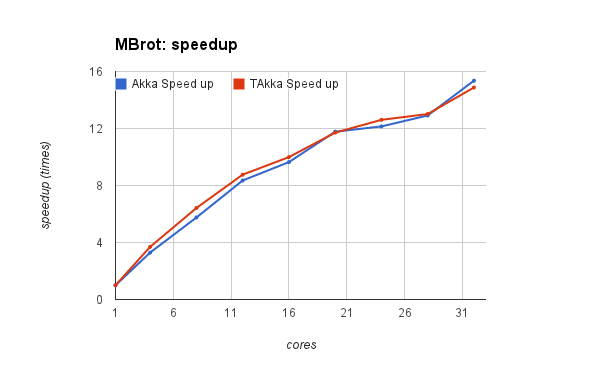
\includegraphics[scale=0.33]{MBrot_speedup.png}
        }\\
        \subfigure[]{
            \label{fig:third}
            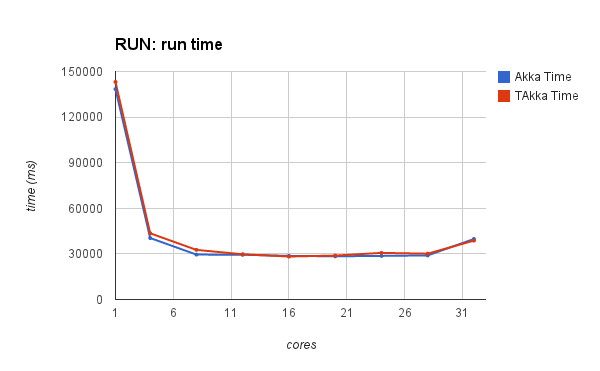
\includegraphics[scale=0.33]{RUN_time.png}
        }
        \subfigure[]{
            \label{fig:fourth}
            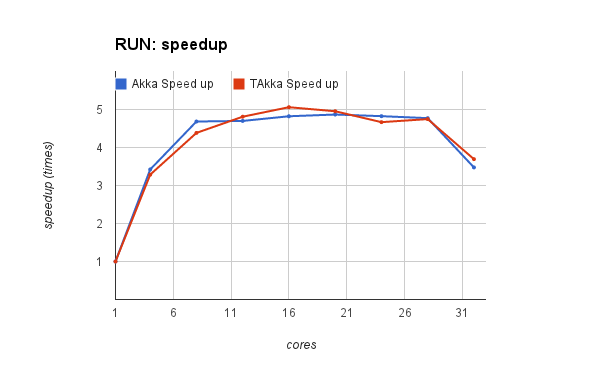
\includegraphics[scale=0.33]{RUN_speedup.png}
        }\\
        \subfigure[]{%
            \label{fig:fifth}
            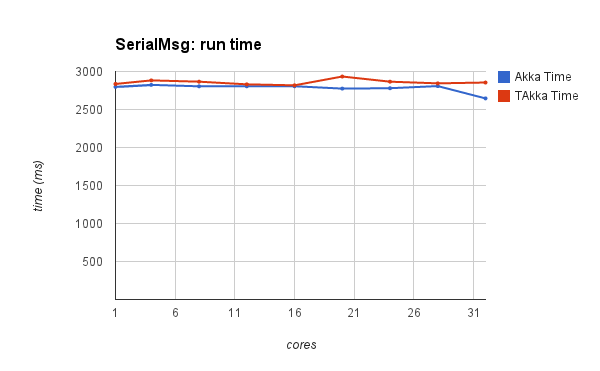
\includegraphics[scale=0.33]{SerialMsg_time.png}
        }
        \subfigure[]{%
            \label{fig:sixth}
            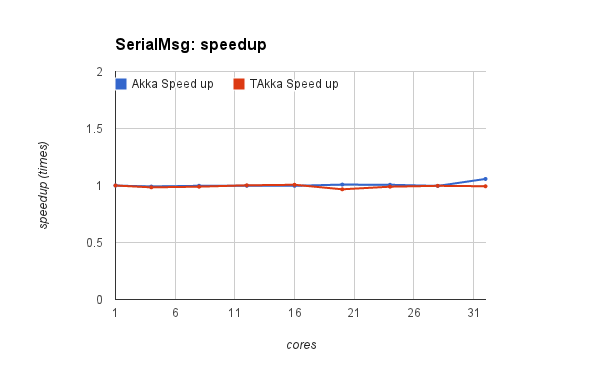
\includegraphics[scale=0.33]{SerialMsg_speedup.png}
        }\\
    \end{center}
    \caption{Efficiency and Scalability Benchmark}
   \label{scalability}
\end{figure}



\section{Conclusion}

Programs written in Actor Model should be easy to reason their intentions
\cite{Hewitt:1973}.  Unfortunately, actors in Erlang and Akka accept
dynamically typed messages and therefore have vague contracts with their outside
world.  The TAkka library introduces a type-parameter for actor-related class.
The additional type-parameter specifies the intention of that actor's solo
communication interface. More importantly, with the help of type-parametrized
actors, the implementation of an actor can be statically checked against the
intention of that actor.

In addition to eliminating programming bugs and type errors, programmers would
like to have reliable failure recovery mechanisms for unexpected run-time
errors.  Supervision tree \cite{OTP} is such a mechanism that has improved the
reliability of a large telecom system written in Erlang.  We are glad to see
that type-parametrized actors can form supervision trees in the same way as
regular actors.

Lastly, tests show that building type-parametrized actor on top of Akka actor
does not introduce significant overheads, respecting to program size,
efficiency, and scalability.  The above test result is encouraging in the sense
that a large amount of previous actor library implementation could be re-used.
We expect similar results could be obtained in other OTP-like libraries such as
the future version of CloudHaskell.


% \acks

% Acknowledgments



\bibliographystyle{plain}
\bibliography{Jiansen}

\appendix
%\section{The TAkka Library}
\label{actor}

An \textit{actor} is a lightweight process that responses to \textit{message}s according to its \textit{behavior}.  In a fault tolerant system, related actors are supervised by their \textit{supervisor}s and form a tree structure.  To better benefit from the functional nature of the actor model, the Akka framework \cite{akka_doc, akka_api} decides to shield actors from the outside using \textit{actor reference}s, which can be freely passed across applications and distributed nodes.

Following core operations are required by the actor model:
\begin{itemize}
  \item \textbf{create}: create an actor and return an actor reference to the actor created;
  \item \textbf{send}: send a message to an actor via its actor reference;
  \item \textbf{become}: update the \textit{behavior} of an actor.
\end{itemize}

Following sub-sections will explain how the TAkka library supports the actor model described above.  APIs of this library is largely influenced by the Akka framework \cite{akka_api}.  Key differences between this library and Akka will be explained in related sub-sections.  Full TAkka APIs are given at \url{http://homepages.inf.ed.ac.uk/s1024484/takka/}.

\subsection{Actor}
\label{sec_actor}

\begin{lstlisting}
package actor
abstract class Actor[Msg:Manifest]{
  protected def typedReceive:PartialFunction[Msg, Unit]
  protected def possiblyHarmfulHandler:akka.actor.PossiblyHarmful => Unit

  protected[actor] implicit val typedContext:ActorContext[Msg]
  implicit final val typedSelf:ActorRef[Msg]
  final lazy val typedRemoteSelf:ActorRef[Msg]

  def preStart():Unit
  def postStop():Unit
  def preRestart(reason:Throwable, message:Option[Msg]):Unit
  def postRestart(reason:Throwable):Unit
}
\end{lstlisting}

The \textbf{Actor} class provides essential constructs for defining an actor.  The \textit{behavior} of an actor is defined by the \textit{typedReceive} method and the \textit{possiblyHarmfulHandler} method.  Users must implement \textit{typedReceive} which will be used as the handler for receiving messages of type \textbf{Msg}.  General users do not have to override the default implementation of \textit{possiblyHarmfulHandler}, which reacts to system messages.  This library uses the same system messages as the akka library \cite{akka_api}.  Selected system messages will be explained in related sections.  In the case that there is an intersection of \textbf{M} and \textbf{PossiblyHarmful}, message of the intersect type will be handled by \textit{typedReceive}.

An \textbf{Actor} instance has fields representing its actor reference(\S\ref{sec_actor_ref}) and actor context(\S\ref{sec_actor_context}).  The \textit{typedSelf} field, initialised at the same time as the actor, is an actor reference that enables local communication to this actor.  Using the value of \textit{typedSelf} at a remote site will usually fail to delivery messages, unless the actor is deployed as a remote actor (\S\ref{sec_actor_system}).  On the other side, value of the \textit{typedRemoteSelf}, if it exists, can be passed around local and remote sites and behave as expected.  Notice that \textit{typedRemoteSelf} is a lazy initialised field.  When \textit{typedRemoteSelf} is first called, a \textbf{NotRemoteSystemException} may raise if the actor is not located in an actor system that supports remote communication.  The use of actor context will be explained in \S\ref{sec_actor_context}.

Moreover, users can specify procedures which will be called 
\begin{inparaenum}[(i)]
\item before the actor is started;
\item after the actor is terminated;
\item before the actor is restarted due to an Error or Exception raised when handling a particular message; and
\item after the actor is successfully restarted.
\end{inparaenum}

Finally, unlike the akka design, this library deprecates the \textit{sender} field which represents the sender of the last receiving message.  The \textit{sender} field is deprecated for several reasons.  Firstly, the type of the \textit{sender} field should be a super type of the union of types of all possible senders expecting a reply.  Therefore, it is still possible to reply a sender with messages of wrong types.  Secondly, without due care, using the shared variable \textit{sender} may introduce bugs in concurrent processes.  Thirdly, experience shows that using \textit{sender} contributes to the difficulty of tracing dataflow in debugging process.  Lastly, to reduce side-effects of message processing, the library designer argues that resources that may effect the message processing, including the sender of a synchronous request, should be part of the message.

%% Actor Reference
\subsection{Actor Reference}
\label{sec_actor_ref}
\begin{lstlisting}
@serializable
@SerialVersionUID("ActorRef-v-0-1")
abstract class ActorRef[-Msg : Manifest]{
  def ![M](message: Msg):Unit
  final def tell(msg: Msg): Unit

  def isTerminated : Boolean
  def path : akka.actor.ActorPath
  final def compareTo (other: ActorRef[_]):Int
}
\end{lstlisting}

As mentioned earlier, same as in the akka library, actors are shielded from the outside using actor references.  Users send messages to an actor via calling the \textit{tell} method or the ! method of corresponding actor references.

Same as in the akka API, the \textit{isTerminated} test of an actor reference checks the liveness of its representing actor.  The \textit{isTerminated} test returns true only if the representing actor is completely shut down by its actor system; temporary actor failure will not change the test result from true because actor is always be supervised and could be restarted after the failure.

In addition, users could enquiry and compare the paths of actor references.  Actor path in this library is not type parametrised because it is not directly related to message sending.

The two serialization annotations before the class declaration ensures that an actor reference could be serialized and deserialized consistently.

\subsection{Actor Reference Configuration}
\label{props}

\begin{lstlisting}
object Props{
  def apply[T, A<:Actor[T]] (implicit arg: ClassManifest[A], t:Manifest[T]): Props[T]
  def apply[T:Manifest](actorClass: Class[_ <: Actor[T]]): Props[T]
  def apply[T:Manifest](creator: => Actor[T]): Props[T]
}
case class Props[-T:Manifest] (props: akka.actor.Props)
\end{lstlisting}

Trying to be consistent with the akka library, this library also provides a Props class, whose instance represents the configuration of actor creation, used in \textit{ActorSystem.actorOf} and \textit{ActorContext.actorOf}.  This section will only look at ways of creating an instance of Props.  Using a Props to create an actor and actor reference will be explained the the next two sections.

\begin{lstlisting}
class StringActor extends Actor[String] {
  // class implementation
}
\end{lstlisting}

Suppose an actor based string processor, \textbf{StringActor}, is implemented as above, users can then obtain a corresponding Props of \textbf{StringActor} using one of the following idioms:

\begin{lstlisting}
  val props = Props[String, StringActor]
  val props = Props[String](StringActorClass)
  //where StringActorClass is a class object for StringActor
  val props = Props[String](new StringActor)
\end{lstlisting}

Omitting the String parameter in above examples will give an actor creation configuration of type Props[\_], whose corresponding actor reference will not accept message of any type.

Though it is more flexible to create a Props by providing a type parameter and an akka Props instance, props object created in this way looses the guarantee of having a correct type parameter captures the type of expecting messages.

\subsection{Actor Context}
\label{sec_actor_context}
\begin{lstlisting}
abstract class ActorContext[M:Manifest] {
  val props:Props[M]
  def typedSelf : ActorRef[M]
  implicit def system : ActorSystem

  def receiveTimeout : Option[Duration]  
  def resetReceiveTimeout(): Unit
  def setReceiveTimeout (timeout: Duration): Unit
  
  def actorOf[Msg:Manifest](props:Props[Msg], name:String):ActorRef[Msg]  
  def actorOf[Msg:Manifest](props:Props[Msg]):ActorRef[Msg]
  def remoteActorOf[Msg:Manifest](props:Props[Msg]):ActorRef[Msg]  
  def remoteActorOf[Msg:Manifest](props:Props[Msg], name:String):ActorRef[Msg]
  def actorFor[E:Manifest](actorPath: String): ActorRef[E]

  def watch[M](subject: ActorRef[M]): ActorRef[M]  
  def unwatch[M](subject: ActorRef[M]): ActorRef[M]

  def become[SupM >: M](behavior: SupM => Unit,    
               possibleHamfulHandler:akka.actor.PossiblyHarmful => Unit)
               (implicit arg:Manifest[SupM]):ActorRef[SupM]
}
\end{lstlisting}

An actor context provides contextual information for an actor.\cite{akka_api}  By accessing an actor context, users could retrieve the props that created the actor, the actor reference that pointed to the actor, the actor system that the actor located in, and the timeout of receiving the first message.  If a timeout is set for the first message, then users should handle the \textbf{ReceiveTimeout} message inside the \textit{possiblyHarmful} method.

Two main usages of actor context are creating and looking for a child actor.  Actor is created by calling the \textit{actorOf} method or the \textit{remoteActorOf} method.  The actor reference returned by the \textit{actorOf} method may not contain a global aware path.  The actor reference returned by the \textit{remoteActorOf} method, on the other hand, can be used at a remote site if the actor system supports remote communication.  Actor created by either methods is supervised by the actor captured by this actor context.  Like in akka, an actor will be given a name at the time of its creation.  If the user does not provide a name, a system generated name will be provided; if the user provides a name which has been used by a sibling of the creating actor, an \textbf{InvalidActorNameException} will be thrown.  Once a valid name is associated with the created actor, a new actor path is generated with the name appending to the actor captured by the actor context.  In another word, a child actor is created.  The \textit{actorFor} method returns an actor reference associated with the provided actor path and the expecting message type.  The returned actor reference will point to a \textbf{DeadLetters}, which is the sink of messages to dead actors, in the case that the actor path is not associated with an actor, or the actor at the actor path has an incompatible type parameter to the provided type parameter.

Like in OTP\cite{OTP} and akka\cite{akka_doc}, an actor could linked to another actor, watching for its death message, or unlinked from a linked actor.  The death message, \textbf{Terminated (actor: ActorRef)}, is handled by the \textit{possiblyHarmful} method of an actor.

Unlike in the akka library, the actor context in this library does not manage information about the current processing message such as its sender.  Any information that the message receiver needs to consider should be part of the message itself.

Finally, this library provides code swap on the actor behaviour using $become$ in the same fashion as in akka.  The current API is different from the akka version in three aspects.  Firstly, the $become$ method in this library requires a handler for system messages.  Fortunately, in most cases, users use actor context inside an actor definition; therefore, users could pass the system message handler retrieved from the actor definition, if the handler does not need to be changed.  Secondly, the behavior parameter has type \textbf{SupM $\Rightarrow$ Unit}, where \textbf{SupM} is usually not \textbf{Any}.  Thirdly, this library deprecated the \textit{unbecome} method to avoid potential problems related to type evolution.

\subsection{Actor System}
\label{sec_actor_system}
\begin{lstlisting}
object ActorSystem {
  def apply():ActorSystem
  def apply(name: String): ActorSystem
  def apply(name: String, config: Config): ActorSystem
}

abstract class ActorSystem {  
  // members with type parameter
  def actorOf[Msg:Manifest](props:Props[Msg]):ActorRef[Msg]  
  def actorOf[Msg:Manifest](props:Props[Msg], name:String):
  def remoteActorOf[Msg:Manifest](props:Props[Msg]):ActorRef[Msg]  
  def remoteActorOf[Msg:Manifest](props:Props[Msg], name:String):ActorRef[Msg]  

  def actorFor[Msg:Manifest](actorPath: String): ActorRef[Msg]  
  def actorFor[Msg:Manifest](actorPath: akka.actor.ActorPath): ActorRef[Msg]

  def deadLetters : ActorRef[Any]

  // members that same as akka version
  def awaitTermination (): Unit 
  def awaitTermination (timeout: Duration): Unit
  def eventStream : akka.event.EventStream
  def extension [T <: Extension] (ext: ExtensionId[T]): T  
  def isTerminated : Boolean 
  def log : LoggingAdapter  
  def logConfiguration (): Unit
  def name : String
  def registerExtension [T <: Extension] (ext: ExtensionId[T]): T  
  def registerOnTermination (code: Runnable): Unit  
  def registerOnTermination [T] (code: => T): Unit  
  def scheduler : akka.actor.Scheduler  
  def settings : akka.actor.ActorSystem.Settings
  def shutdown (): Unit
  override def toString():String 
  def uptime : Long = system.uptime

  // addtional members for constructing remote ActorRef  
  def isLocalSystem():Boolean
  
  @throws(classOf[NotRemoteSystemException])
  def host:String
  
  @throws(classOf[NotRemoteSystemException])
  def port:Int
}

case class NotRemoteSystemException(system:ActorSystem) extends Exception("ActorSystem: "+system.name+" does not support remoting")
\end{lstlisting}

An actor system manages resources to run its containing actors.  Same as the akka library, an actor system is initialised by calling one of the \textit{ActorSystem.apply} methods.  Users could optionally provide a name and a configuration when creating an actor system, otherwise a default name and a default configuration will be provided.  Actor system created with the default configuration can only provide actor references for local communication.  In a user defined configuration, remote communication and other functionalities may be enabled.  For more information about the \textbf{com.typesafe.config.Config} object and actor system configuration, users may refer to the akka API\cite{akka_api} and the akka documentation\cite{akka_doc}.  A later version of the type-parametrised actor library may provide a convenient API for writing actor system configuration or enable remote communication by default.

\S\ref{sec_actor_context} explains how to created an actor supervised by another actor.  To construct a complete supervision tree inside an actor system, a top-level actor needs to be created.  The akka library \cite{akka_doc} provides an guardian actor, \textit{user}, for all user created top-level actors.  This library follows the same design and put actors created using \textit{ActorSystem.actorOf} and \textit{ActorSystem.remoteActorOf} at the next level of the \textit{user} actor.

This library also provides a typed version of \textit{deadLetters}, which is the receiver of messages to stopped or non-exist actors.  The last two methods in the \textbf{ActorSystem} class are implemented to help constructing actor references that can be used at remote sites.  The isLocalSystem returns false if the actor system is registered to a host name and port number, or returns true otherwise.  The rest methods have the same functionality as their corresponds in the akka library\cite{akka_api}.

\subsection{FSM}

\begin{lstlisting}
object FSM {
  case class CurrentState[S, E](fsmRef: ActorRef[E], state: S)
  case class Transition[S, E](fsmRef: ActorRef[E], from: S, to: S)
  case class SubscribeTransitionCallBack[E](actorRef: ActorRef[E])
  case class UnsubscribeTransitionCallBack[E](actorRef: ActorRef[E])
  case class Timer[E](name: String, msg: E, repeat: Boolean, generation: Int)
                       (implicit system: ActorSystem) 
}

trait FSM[S, D, E] extends akka.routing.Listeners {
  this: Actor[E] =>

  type State = FSM.State[S, D]
  type StateFunction = scala.PartialFunction[Either[Event[E], StateTimeout.type], State]
  type EventFunction = scala.PartialFunction[Event[E], State]
  type TimeoutFunction = scala.PartialFunction[StateTimeout.type, State]
  
  protected[actor] def setTimer(name: String, msg: E, timeout: Duration, repeat: Boolean): State
  protected final def when(stateName: S, stateTimeout: Duration = null)(eventFunction: EventFunction): Unit
  protected final def whenStateTimeout(stateName: S, stateTimeout: Duration = null)(timeoutFunction: => State): Unit
  case class Event[E](event: E, stateData: D)
}

trait LoggingFSM[S, D, E] extends FSM[S, D, E]
\end{lstlisting}

Whenever possible, the library designer suggests to avoid using mutable actor state so that the actor behavior will be more functional and more likely to be effect free.  In some cases; however, if a stateful actor better captures a problem, the user may consider encode the actor as a finite state machine (FSM) using the typed \textbf{FSM} trait.

Like what has been done in the Actor class, a generic type denoting the type of events is added to the FSM trait comparing to the akka version.  To save the space, the above list only gives public members with restricted type.  The rest of members have the same signatures as members in the akka version.

\begin{comment}
%% Library Implementation
\section{Library Implementation}
\label{implementation}

\subsection{Programming Patterns for the Implementation}
To reuse the significant amount of work done in the akka project \cite{akka_doc} and provide consistent yet better typed APIs, most classes in \S\ref{actor} are implemented using the delegation pattern, employing a suitable akka instance as the value of an immutable field.  Unfortunately, the delegation pattern cannot be applied to both \textbf{Actor} and \textbf{ActorContext} as they are initialised simultaneously in a special way in the akka implementation.  To resolve the deadlock when initialising an actor, the library designer decided to implement the \textbf{Actor} class via inheritance.  Using inheritance means all poorly typed features in the akka \textbf{Actor} are inherited to the type-parametrised actor library.  Fortunately, different from using members in the \textbf{ActorContext} class, using members in the \textbf{Actor} class usually not effects the outside of an actor.  The library designer further provides an implementation for the protected \textit{receive} method inherited form the akka \textbf{Actor} class.  By doing this, an explicit \textbf{override} annotation is required if a user would like overrides the implementation of \textit{receive} method for a good reason.


\subsection{Code and Type Evolution}
\label{type_evolution}
Erlang/OTP \cite{OTP} provides a sophisticate mechanism for hot code swap on any OTP process via the code\_change/3 function.  In akka, hot code swap is only partly supported for actor behaviors via pushing or popping handlers to and from a handler stack.  Although a \textbf{Wrapper} class has been implemented for simulating Erlang/OTP style hot code swap, it is not used in the current implementation which is aiming at providing  APIs similar to those in the akka library.

\begin{lstlisting}
  def become[SupM >: M](behavior: SupM => Unit,    
               possibleHamfulHandler:akka.actor.PossiblyHarmful => Unit)
               (implicit arg:Manifest[SupM]):ActorRef[SupM]
\end{lstlisting}

Notice that the type-parametrised library does no have the \textit{unbecome} method but have a \textit{become} method has signature given as above.  The library does not provide the \textit{unbecome} method because the library designer would like to ensure that code evolution is always backward compatible.   For the same reason, the new behavior of an actor must not cover less types of messages.

Furthermore, after calling \textit{become[SupM](behavior, pHH)}, users would expected a way to retrieve actor reference of type \textbf{ActorRef[SupM]}.  For this matter, \textit{become} returns an actor reference rather than \textit{unit}.  In addition to passing the returned value of the \textit{become} method, users can retrieve the wilder typed actor reference via \textit{actorFor} method in \textbf{ActorContext} and \textbf{ActorSystem}.

As the type of actor reference may evolve at the run-time, an immediate question is how to interpret the meaning of the static type parameter for the class definition.  The library designer suggests that the type of \textbf{Actor}, \textbf{ActorContext}, \textbf{Props}, and the \textit{typeSelf} field, etc. only denotes the most precise type of expecting messages of the $initial$ actor, i.e. the first actor initialised by an actor definition.

Users of this library would expected the type parameter of \textbf{Actor}, \textbf{ActorContext}, and \textbf{Props} classes is a contravariant type.  Unfortunately, the type parameter of the \textit{become} method, \\ \textbf{SupM $>$: M}, put the class type parameter, \textbf{M}, at a covariant position.  There are two workarounds to this issue:
\begin{enumerate}[1)]
\item Change the type parameter of \textit{become} to \textbf{SubM $<$: M}.  As a consequence, users cannot upgrade the actor behavior to an handler which is able to deal with more types of messages.
\item Keep the current signature of the \textit{become} method.  Except for the \textbf{ActorRef} class and the \textbf{Props} class, remove the contravariant restriction of the type parameter of related classes.  
\end{enumerate}

This library adopted the second solution.  Fortunately, it does not cause problems in practice.  In most cases, as actors are shielded from actor references, users are more interested in the type of an actor reference rather than the full type of the represented actor.  To retrieve an actor reference which is capable to send messages, users could try to query on the \textit{actorFor} method, or the typed name server introduced in \S\ref{name_server}.  The only difficulty is constructing a less general actor from a general purpose actor class.  The trick is to initialise an internal general purpose actor and delegate received messages to that actor.

\subsection{Actor Reference with Global Awareness}
As mentioned in \S\ref{sec_actor_context}, most actor references retrieved by akka APIs cannot be used at remote sites.  There are three exceptions to the above argument:
\begin{inparaenum}[(i)]
\item the $sender$ of messages sent from a remote site;
\item the actor reference to an actor that is configured to be deployed at a remote actor system; and
\item the actor reference retrieved by $actorFor(path:String)$ where host name and port number are specified as part of the actor path.
\end{inparaenum}  The $sender$ field in case (i) has been deprecated in the typed-parametrised actor library.  From the provided akka API, actor references retrieved in case (ii) cannot be distinguished from local actor references retrieved using the same $actorOf$ method.  Actor references retrieved in case (iii) supports remote communication; however, manually manage host name and port number is a trivial task.  To reduce the work of host name and port number management, the type-parametrised actor library provide new supports for retrieving actor reference with global awareness.
\end{comment}


%%\section{Project Progress and Plans}

\subsection{Progress Achieved since the First Panel Review}

With suggestions from panel members, I have been working on the more focused aim stated in \S\ref{aim}.  Research objectives are also tailored to more specific tasks accordingly.  Meanwhile, I studied more related works on concurrent programming and type theories.

Before the new year, three medium-sized applications has been identified.  Both the ATM example and the main application of the elevator controller example have been ported into Scala using akka libraries.  The later example contains an interface for properties checking using QuickCheck.  I am working on porting QuickCheck properties specified in the Erlang version to my Scala implementation.  The porting of a larger example, Riak, will be started soon.

For the work of implementing a prototype Scala library that supports OTP principles, I found a way of mimicking hot code swap via object delegation.  However, this strategy requires at least one non-swappable wrapper process, which is not needed in the Erlang/OTP platform.  I also identified some problems of implementing actors which have a type parameter that specifies the type of expecting messages.  To overcome the bottleneck of solving those problems, I postponed this work for learning lessons from the design of existing frameworks.

In the last report, I mentioned Walder's “type pollution” problem when using the Actor model to construct layered systems.  One solution is using subtyping on the type parameter of the reference to a typed actor.  However, this solution is awkward and does not cope with the dynamic configuration of distributed systems.  To improve this situation, I recently proposed using union types to plot a type in a type hierarchy on the fly. At the meantime, Professor Walder pointed out that another solution could be using session types, where each channel is only used for the communication between two parties.

\subsection{Plan for the Second Year}
In the rest of the second year, I will port the Riak example and summarise problems that I encountered when translating the three examples into Scala using akka.  More translation exercises will be done if proper examples are found.

Based on the summary, I shall started the the design and implementation of library that supports OTP principles.  This work will require iterative and incremental development on requirement analysis, interface design, functionality implementation, and system evaluation.  In addtion, a flexible plan should be given in advance to guide and monitor the pace of progress.

\subsection{Plan for the Third Year}
The beginning of the third year will continue the work of library implementation. After that, the library will be published with a technical report that covers:  
\begin{inparaenum}[(i)]
  \item functionalities provided by the library,
  \item alternative choices of library design and reasons for adopting the chosen design,
  \item benchmark results of selected canonical distributed applications.
\end{inparaenum}  

In the meantime of receiving feedbacks from programming communities, I will re-implement the selected applications with the new library.  Testing results for the new implementation will be published in an updated version of library documentation.

Finally, as promised in the research objectives, a more comprehensive summary of common challenges in distributed programming and their solutions will be given.  The summary will reveal how language libraries, which is used for practical purposes, are related to their theoretical guidance underneath.  It may also plot research blanks for future study.


\subsection{Potential Risks}
As a novel and ambitious research, some tasks may be tougher than my expectation.  Also, results of some tasks may differ from my intuition.  Risk analyses for planed objectives are given below.d

Firstly, sample applications used in the first and second objectives, which are the basis of research problems specification and results evaluation, must be carefully selected.  It would be better to select open-source applications implemented in high-quality code.  For a candidate application, we need to analysis the proportion of implementation for OTP features to the implementation for other problems out of our main research interests.  Fortunately, we have identified three appropriate applications.

Secondly, some research problems rooted in the center of distributed programming, and therefore is inevitably also investigated by other researchers.  Although it seems feasible to re-implement identified applications in other frameworks and then identify problems of using those frameworks, our chosen comparing frameworks are vigorous and evolving quickly.  For example, significant changes have been made to the actor model in the new akka library (version 2.0).  The evolving of comparing frameworks contributes to plausible solutions to some research problems as well as pressures of providing devised simpler solutions for tough problems.  In addition, since there is no uniform model for distributed programming, it would be hard to evaluate to what extend our library interface is a general framework for distributed programming.

Lastly, apart from above general difficulties, I also encountered implementation difficulties listed in \S\ref{problems}.  At the time of this writing, it is not clear to me how those problems could be solved in a neat way.  I anticipate that new problems will be added to the list when I write more programs in type safe-less environment.

Despite the identified and potential troubles which may distract this research from a perfect result, none of above risks should be the principle hindrance of achieving the main objectives listed in \S\ref{objectives}.  With proper plans, wide sources of suggestions, and the commitment to research objectives, the proposed research should be suitable for a PhD project.

\end{document}
